\section{\textsf{Rear:} a framework for virtual exocentric vision systems}
\label{sec:rear}

In this chapter we will describe \textsf{R.E.A.R.} - 
\textit{Rear Exocentric Augmented Reality}, a framework 
for the development of virtual exocentric vision systems.
%
It has been written in C++, following an object-oriented 
approach, and implements the minimal set of tools and functionalities 
needed to create representations of a mobile robot in its environment 
through the use of augmented reality techniques, as described in 
section \ref{sec:exo}.
%

%
For what concerns graphics, \textsf{R.E.A.R.} relies on OpenGL.
It makes use of three software components: a \textit{camera}, 
a 3D model of the \textit{robot} itself and a \textit{texture}.
%
The camera provides the user with a view of the OpenGL space 
from a certain point-of-view and with a certain field-of-view. 
It identifies a \textit{viewing frustum} - as shown in figure 
\ref{fig:openglspace} - whose volume corresponds to the 
portion of OpenGL space displayed on the user's screen.
%
To give the user the illusion of seeing the robot from an 
external point-of-view, the 3d model of the robot is drawn 
within the viewing frustum, while the more distant frustum base 
is applied a texture displaying a picture previously 
captured from the robot's egocentric camera.
%

%
An example of what a user sees is showed in figure \ref{fig:snap}.
%
\begin{figure}[!h]
  \begin{center}
    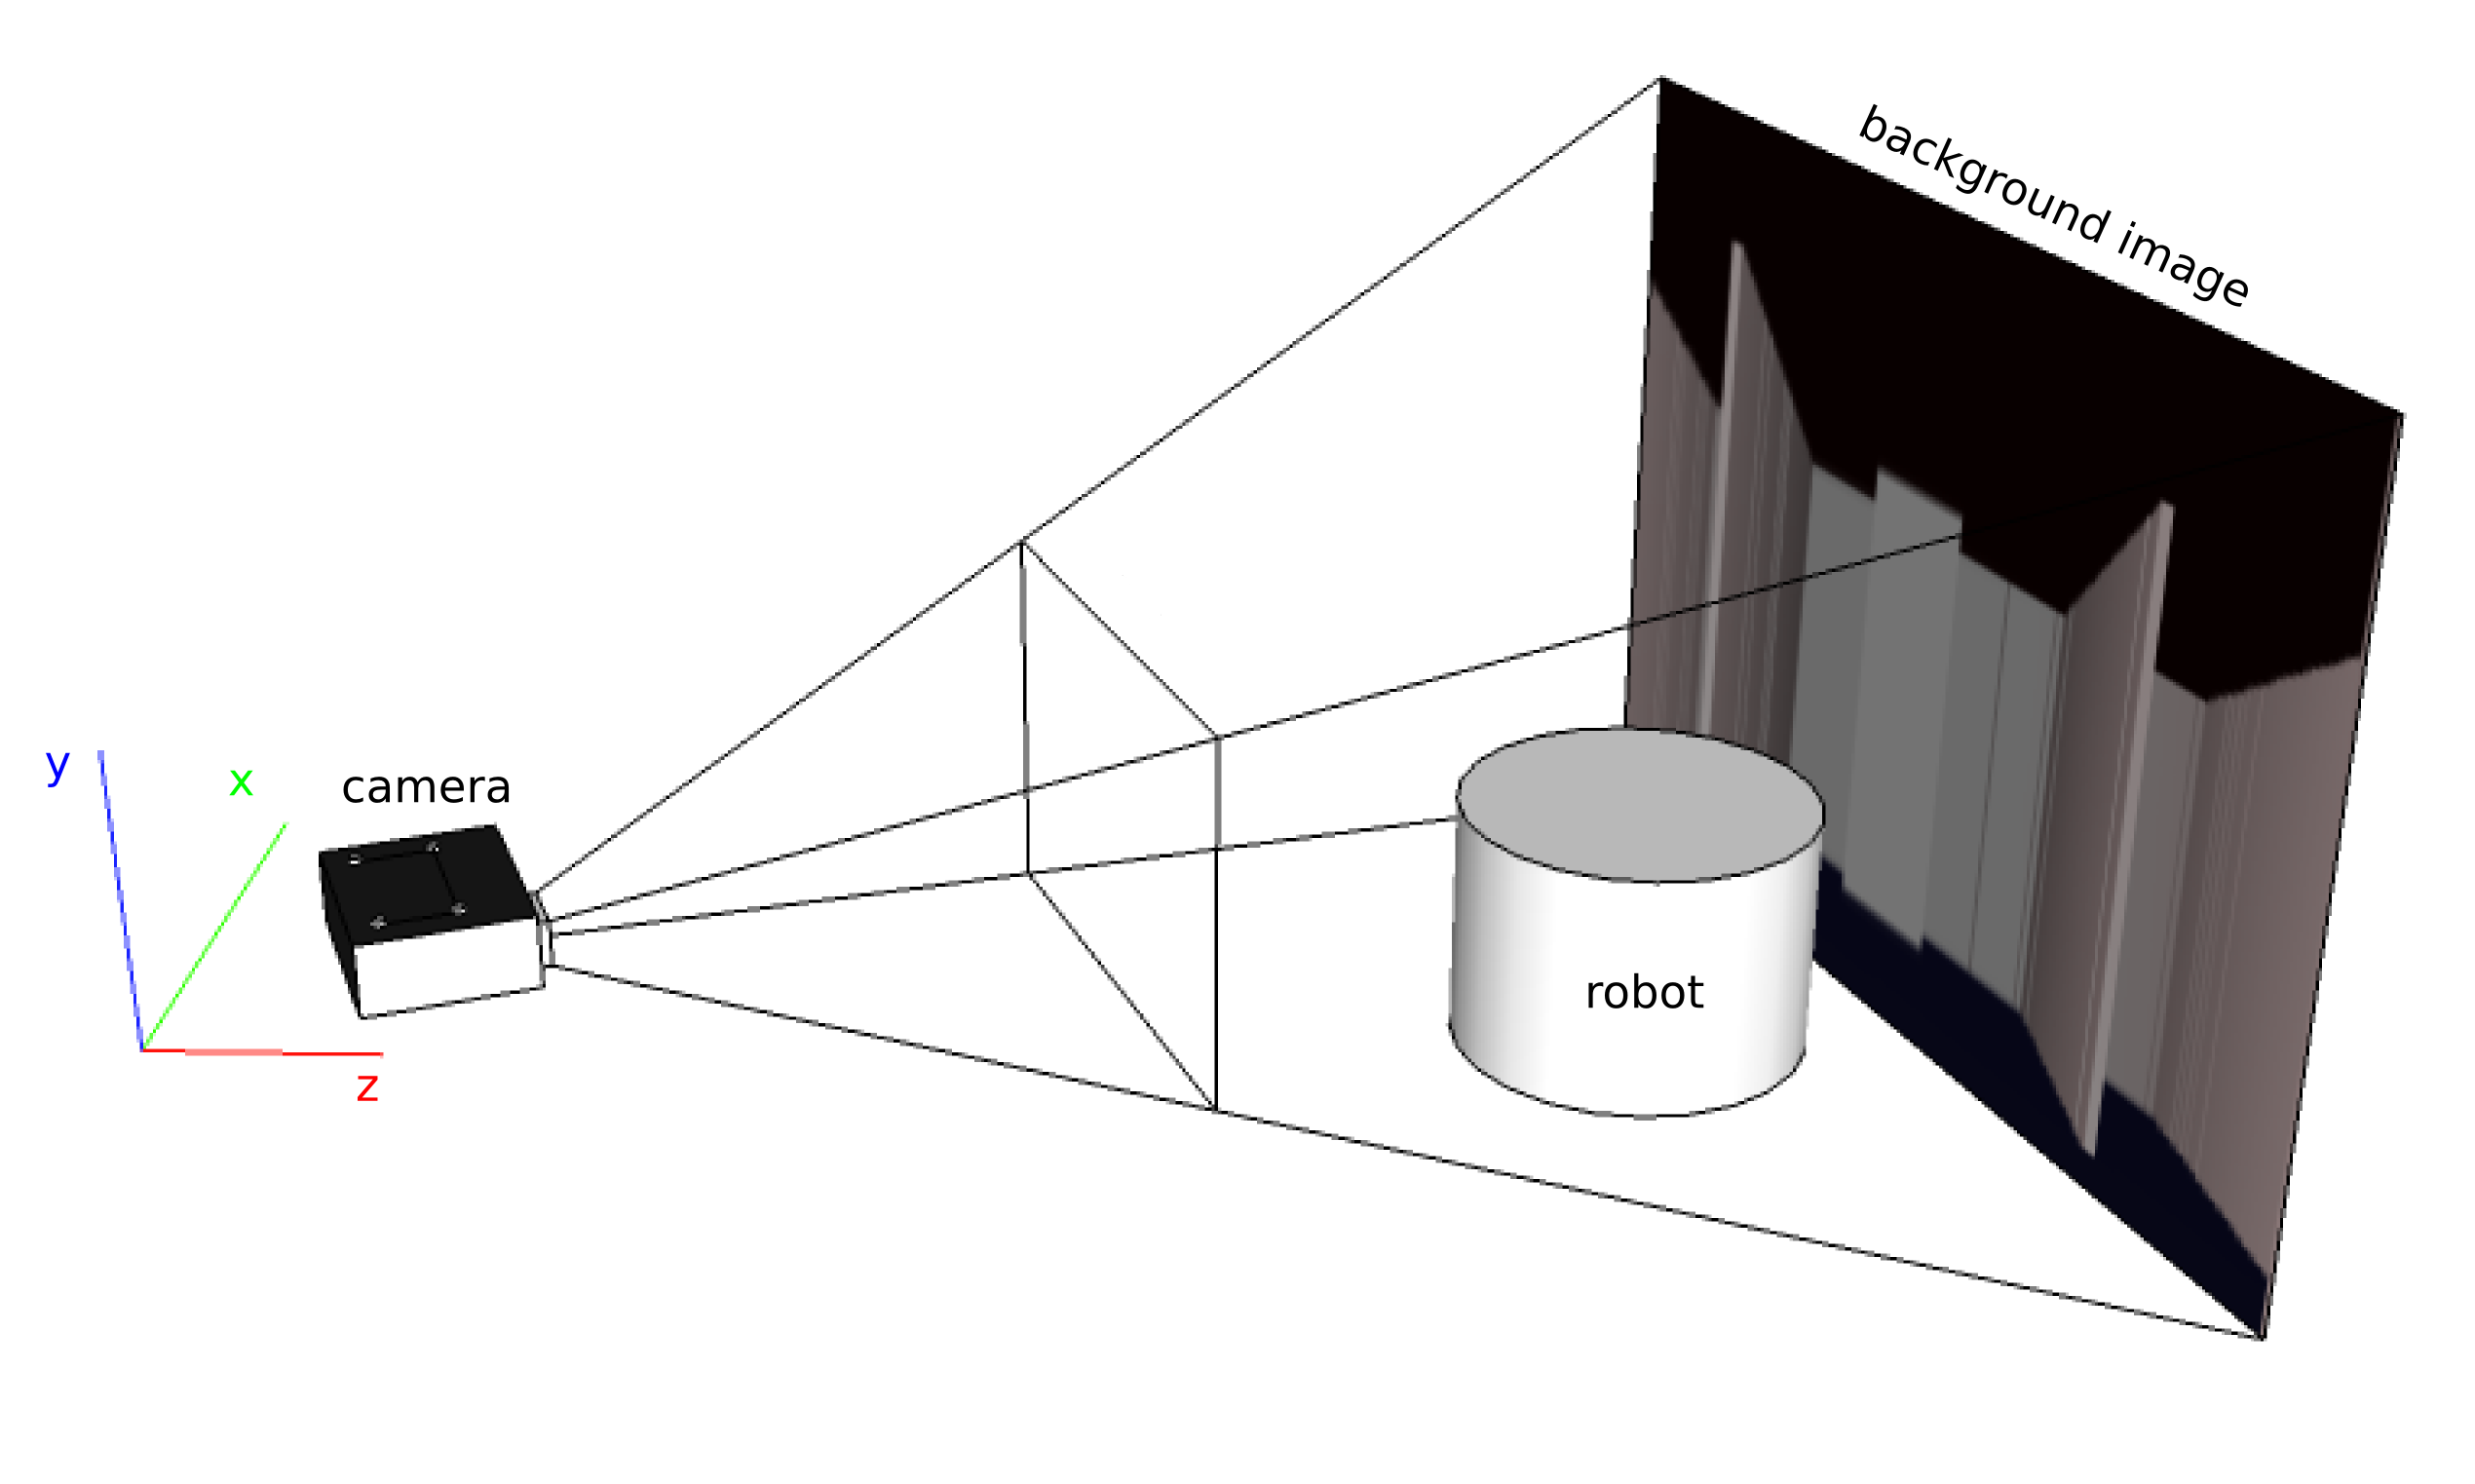
\includegraphics[width=300pt]{img/camera_frustum_scheme.png}
    \caption{The OpenGL space}
    \label{fig:openglspace}
  \end{center}
\end{figure}
%
\begin{figure}[!h]
  \begin{center}
    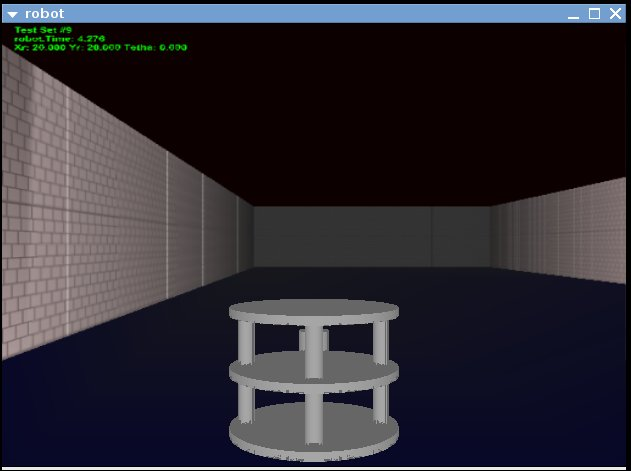
\includegraphics[width=300pt]{img/rear_snapshot_large.jpg}
    \caption{A snapshot from a \textsf{R.E.A.R.}-based application}
    \label{fig:snap}
  \end{center}
\end{figure}
%

%
Main issues in the approch we have just described are 1. 
\textit{where} to draw the robot within the viewing frustum 
and 2. \textit{which} of the captured images is to be used 
as background.
%
For what concerns the first issue, one can intuitively guess 
that the simplest way to determine the robot position 
within the frustum is to know the current robot position 
and orientation and the position and orientation of the egocentric 
camera when the snapshot was taken and, then, to set the 
position of the 3d model of the robot and the point-of-view 
of the camera accordingly.
Well, that's what \textsf{R.E.A.R.} does.
%
Therefore, to run, every \textsf{R.E.A.R.} concrete implementation 
needs, at least:
%
\begin{itemize}
  \item a set of snapshots captured from the robot egocentric camera, 
    together with the robot position at the time it was taken
  \item the robot's current position
\end{itemize}
%
Such data is retrieved every time the operator, using the 
interface provided by \textsf{R.E.A.R.} itself, sends a 
motion command to the robot.
%
Only once new data is collected, \textsf{R.E.A.R.} chooses 
an image to set as background and draw the robot model within 
the frustum. So, for what concerns issue no. #2, as already 
underlined in \cite{sugimoto}, let us say that there is not 
a \textit{unique} way to determine which image is to be set 
as background, since different image selection algorithms 
would differently affect user perceptions and. We will have a 
deeper look at some image selection algorithms in section
\ref{sub:howbackgroundimage}.
%
Finally, the overall execution loop is resumed by the flowchart showed 
in figure \ref{fig:overall_diagram}.
%
\begin{figure}[!h]
  \begin{center}
    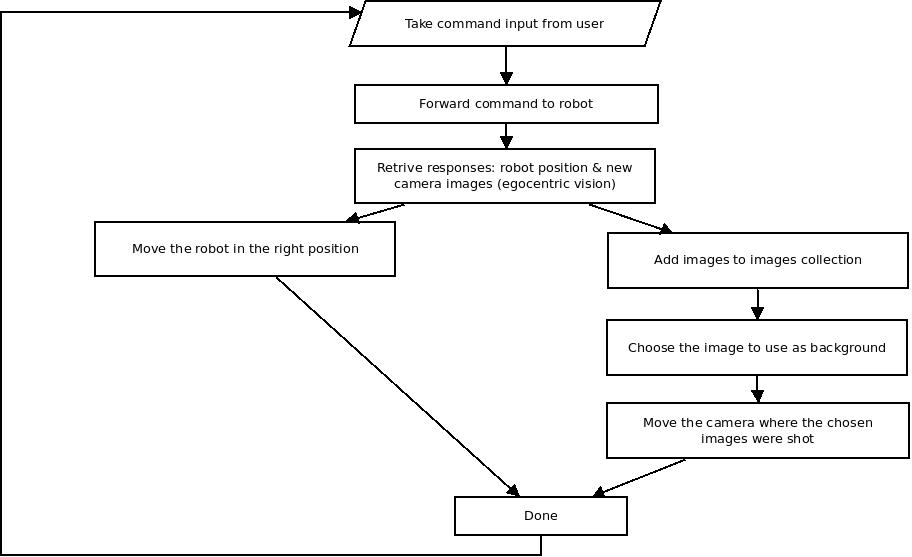
\includegraphics[width=350pt]{img/overall_diagram.jpeg}  %robot pic
    \caption{Application flowchart}
    \label{fig:overall_diagram}
  \end{center}
\end{figure}
%
%% The overall schema can be resumed by the following diagram (see figure
%% \ref{fig:overall_diagram}). User sends a command to the exocentric vision
%% application, in order to guide the robot through the remote environment.
%% The exocentric vision application forwards the command to the robot or the
%% simulator (paragraph \ref{sec:simulator}) and waits for the response.
%% The latter includes the new robot position and the new egocentric camera images.
%

%
%% All the egocentric camera images retrieved are stored in a data set and coupled
%% with robot coordinates and orientation at the moment when they were shot. Going
%% on with the application a large collection of egocentric images will be gathered.
%% %
%% Since every image owns its data about position and orientation when shot, we can
%% move and point the camera object to obtain the right visual of the external world.
%% Wherever the robot is situated, we will be able to watch it from the right point of view,
%% depending on the texture image chosen.
%% %

%% %
%% All the process explained above is lacking of one part: how to choose the background image,
%% knowing the actual robot position and orientation. If we decided to choose the closest image
%% to the robot we would always show the egocentric vision, because the algorithm would select
%% always the image with the same position and orientation of the robot. The distance between
%% the robot and the selected images would be equal to zero, which is doubtless the minimum possible
%% value.
%% %

%% %
%% The algorithms to take the right image in exocentric vision can be various. Each one has its own
%% advantages and disadvantages, we will chose the one able to guarantee the best trade-off.
%

%
\subsection{Class diagram}
%
Let us have a look at \textsf{R.E.A.R.} class diagram, showed in figure 
\ref {fig:class_diagram}.
%
\begin{figure}[!h]
  \begin{center}
    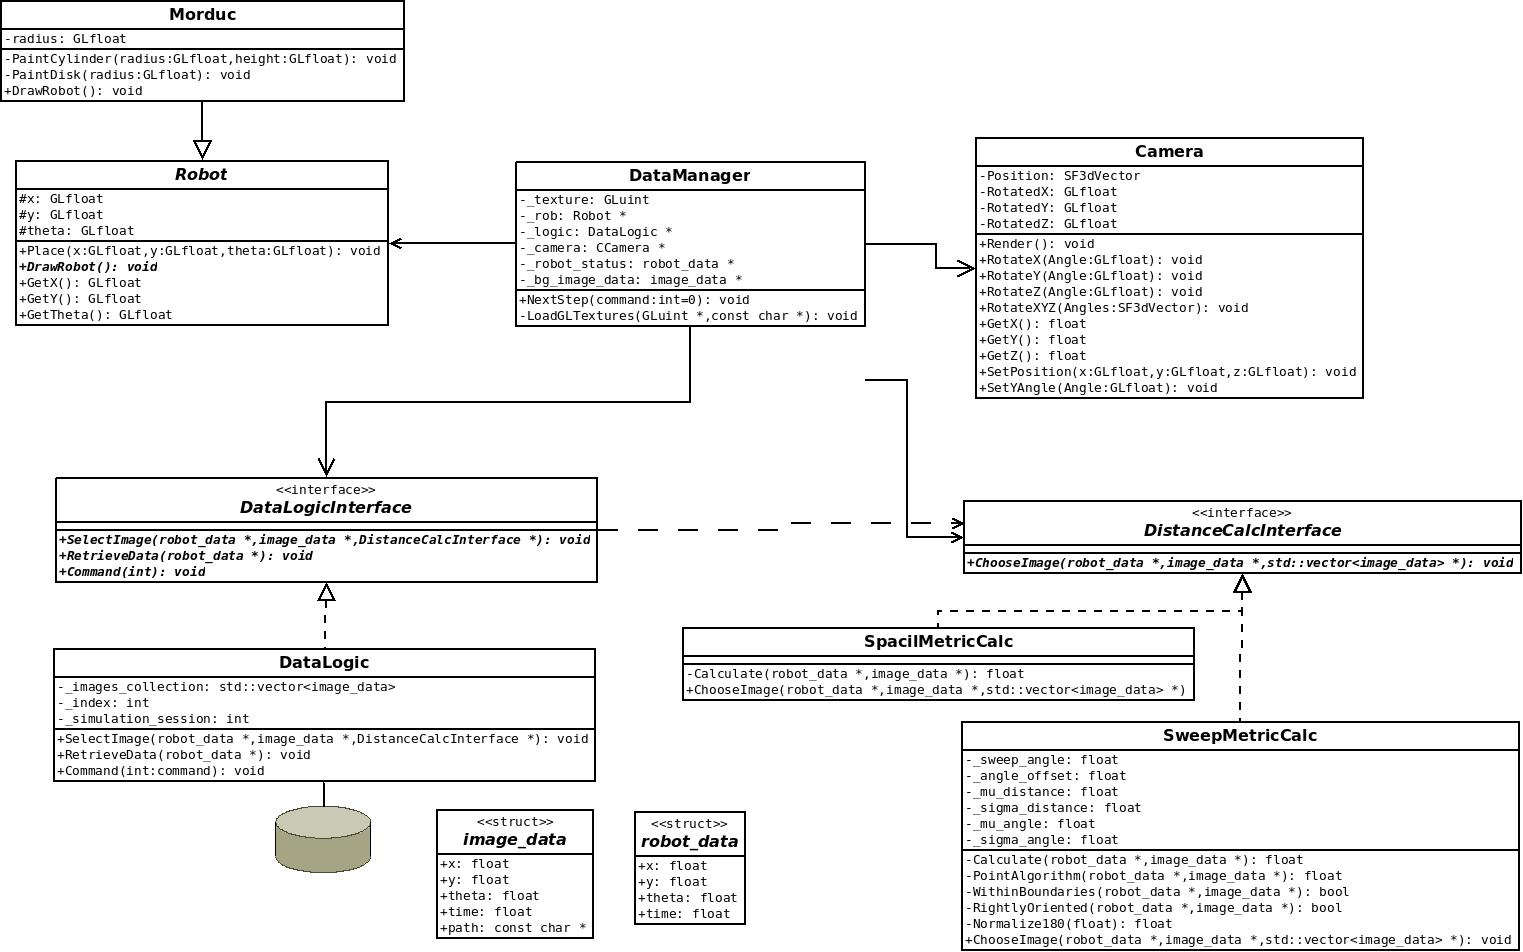
\includegraphics[width=400pt]{img/class_diagram.jpeg}  %robot pic
    \caption{\textsf{R.E.A.R.} class diagram}
    \label{fig:class_diagram}
  \end{center}
\end{figure}
%
It features three main classes: \texttt{Robot}, \texttt{Camera} and 
\texttt{DataManager}. The former is intended to be a
representation of the state of the actual robot. \texttt{Camera} 
is a \textit{helper class}, which provides some methods 
to easily set the point-of-view within any \textsf{R.E.A.R.}
based application. Finally, \texttt{DataManager} is intended to 
be used as the application entry point.
%
The diagram also features two interfaces: \texttt{DataLogicInterface} and
\texttt{DistanceCalcInterface}, they have to be implemented by 
programmers who want to create their own concrete exocentric 
vision system. 
%
Going into details, the former decouples the application 
core, that is the \texttt{DataManager}, from the data source.
This way, \texttt{DataManager} code is totally unaware of 
the technology used to retrieve data from the robot - e.g. 
sockets, web services, etc.
%
\texttt{DistanceCalcInterface}, instead, defines the interface 
of the component responsible for determining which image is the 
\textit{proper} one to be used as background to draw on. In this 
case, the aim of the use of an interface is to leave programmers 
able to implement their own image-choosing algorithms without 
having to change none of the other classes.
%
Now, let us have a look under the hood at the classes we have just 
introduced.
%
%% spiegare come le funzionalita` descritte nell'introduzione si mappano
%% sulle varie classi
\subsubsection{The DataManager Class}
\label{sub:datamanager}
As already stated, the \texttt{DataManger} class represents a global 
access point to the whole application. Its declaration is reported in
listing \ref{code:datamanager_class}.
%
\begin{lstlisting}[caption={DataManager class declaration}, label={code:datamanager_class}, frame=trBL]
class DataManager
{
 private:
  GLuint _texture[1];
  Robot * _rob;
  Camera * _camera;
  DataLogicInterface * _logic;
  DistanceCalcInterface * _calculator;

  robot_data * _robot_status;
  image_data * _bg_image_data;

  /* bind the specified image to a texture */
  void LoadGLTextures(GLuint *, const char *);

 public:
  DataManager(Robot *, DataLogic *, Camera *, 
	      DistanceCalcInterface *); 
  ~DataManager();
  void NextStep();
};
\end{lstlisting}
%
The \texttt{DataManger} is meant to be used as a \textit{singleton}, 
that is, there must be a unique instance of \texttt{DataManager} 
within a \textsf{R.E.A.R.} based application.
%
As its name suggests, \texttt{DataManager} manages and coordinates 
all of the components of the exocentric vision system and, hence, 
keeps a private reference to all of them: 
the \texttt{Robot} unique instance (see section \ref{sub:robotclass}), the 
\texttt{Camera} unique instance (see section \ref{sub:cameraclass}),
a \texttt{DataLogicInterface} object, a \texttt{DistanceCalcInterface} 
object and an OpenGL texture id number.
%

%
Once the application is started, it's \texttt{DataManger}'s duty 
to move robot and camera within the OpenGL space. Moreover, 
it's also responsible for retrieving position data from the actual robot
every time the user asks for it and for asking a \texttt{DistanceCalcInterface}
object to choose one of the images recorded by the robot's 
egocentric camera and for displaying it on the background. 
All of these operations are performed within the \texttt{NextStep()}
method, reported in listing \ref{code:next_step}.
%
\begin{lstlisting}[caption={The \texttt{DataManager::NextStep()} method}, label={code:next_step}, frame=trBL]
void DataManager::NextStep() {

  image_data old_image;

  // save old background image position and orientation
  old_image.x = _bg_image_data -> x;
  old_image.y = _bg_image_data -> y;
  old_image.theta = _bg_image_data -> theta;
  
  // retrieve new position data from the robot
  _logic->RetrieveData(_robot_status);

  // move robot with _robot_status data
  _rob->Place(_robot_status->x,
	      _robot_status->y,
	      _robot_status->theta ); 
    
  // select an image to set as background
  _logic->SelectImage(_robot_status, _bg_image_data,
		      _calculator);

  // if the selected image differs from the previously
  // selected one, move the camera
  if ( old_image.x != _bg_image_data -> x ||
       old_image.y != _bg_image_data -> y ||
       old_image.theta != _bg_image_data -> theta )
    {
      _camera -> SetPosition( _bg_image_data -> x,
			      9.f,
			      _bg_image_data -> y);
      
      _camera -> SetYAngle( _bg_image_data -> theta - 90);
    }

  // actually draw the image in the background
  LoadGLTextures(_texture, _bg_image_data->path);
}
\end{lstlisting}
%
%% The data regarding robot status, camera position or texture image have to be retrieved from other components,
%% in our case other objects. It is for these reason that a \texttt{DataManager} instance owns the references to
%% other two concrete objects, which implement the \texttt{DataLogicInterface} and the \newline
%% \texttt{DistanceCalcInterface}.
%

%
The former is called in order to transfer the next command to the robot (i.e. which way to move) and get the
consequent new robot data (its position and orientation). Every fetched data are coupled with a timestamp value
(see \texttt{robot\_data} struct in figure \ref {fig:class_diagram}). Besides, a concrete objects which implements
\texttt{DataLogicInterface} allows to retrieve information about the image file selected for background
(see \texttt{image\_data} struct, again in figure \ref {fig:class_diagram}). We refer the reader to chapters
\ref{sub:howretrievedata} and \ref{sub:howbackgroundimage} for more details abouts \texttt{DataLogicInterface}'s
abstract method; chapters \ref{sub:datasource} and \ref{sub:metrics} for a concrete example.
%

%
The other reference, pointing to a \texttt{DistanceCalcInterface} implementation, is used to recall the algorithm
whose aim consists in calculating the score value for a single image, given the robot status and image itself. We
remind that a score algorithm has to be implemented in order to choose the proper background image among all the
collected ones, as explained in depth in chapter \ref{sub:howbackgroundimage}.
%

%
Since the unique method present in \texttt{DistanceCalcInterface} (named \texttt{Calculate}) is called by the
concrete instance of \texttt{DataLogicInterface}, \newline \texttt{DataManger} forwards its reference to the latter,
when requested. As before, we refer the reader to chapters \ref{sub:howbackgroundimage} and \ref{sub:metrics} for
more details and some concrete examples.
%

%
By calling the public method \texttt{NextStep}, \texttt{DataManager} forwards the new command to the concrete
\texttt{DataLogicInterface} instance, in order to teleguide the robot and retrieve its new status
(i.e. position and orientation). Acquired new robot data, it is then possible to move the robot in the
right position, by setting the x, y and theta value of the robot class instance (see method \texttt{Place},
present in class \texttt{Robot}, chapter \ref{sub:robotclass}).
%

%
Later on, the concrete \texttt{DataLogicInterface} instance is asked again for the background image. After
retrieving it (or better, the coupled \texttt{image\_data} struct) \texttt{DataManger} instance moves the camera
object to the position where the selected image were shot (see methods \texttt{SetPosition} and \texttt{SetAngle},
both present in class \texttt{Camera}, chapter \ref{sub:cameraclass}), and renders the texture image before ending.
%

%
Next user command implies another calling to the \texttt{NextStep} method and the re-execution of all the steps just
described.

\subsubsection{The Robot Class}
\label{sub:robotclass}

The robot class is the \textsf{R.E.A.R.} internal representation of 
the actual robot. Let us have a look at its declaration,

\begin{lstlisting}[caption={Robot class declaration}, label={code:robot_class}, frame=trBL]
class Robot
{
 private:
  /* position */
  GLfloat x ;
  GLfloat y ;					
  GLfloat theta ;  
  
  /* scale factor */
  GLfloat radius; 

 public:
  Robot(float radius = 4.0f);
  void Place(GLfloat x, GLfloat y, GLfloat theta);
  void DrawRobot();

  GLfloat GetX();
  GLfloat GetY();
  GLfloat GetTheta();    
};
\end{lstlisting}
%
Three of the four private attributes (\textsf{x, y, theta}) 
store the position of the actual robot. The fourth attribute, 
\textsf{radius}

On the one hand, it has private 
attributes which store the robot position every time 
new data is retrieved.
%

%% The robot class, present in Filippo Privitera's simulator 
%% \cite{privitera}, has been simplified and then introduced in
%% exocentric vision control code. In this chapter we will 
%% exam the main differences.
%

%
Both classes represent the 3morduc robot in openGL world. 
This means that the robot class offers, among others, a
method with the purpose of drawing itself, called by the 
OpenGL framework when it is necessary. The operation of 
drawing is completed thanks to other two methods, able 
to draw the elementary part of the robot - e.g. cylinders and disks.
%

%
There are not considerable different between the tho 
drawing method implantation. The main one is that in the 
new method, before starting drawing, the model-view matrix 
is copied in order to restore it at the end of the process. 
In these way we do not affect the model-view matrix status 
by drawing the robot.
%

%
The robot class, after the refactoring process, loses many 
of its public attributes and methods, so in the
exocentric vision control it is much more simple than the 
original one. First of all, the new class does not contain either
attributes to store the actual speed vector component, or 
a chronometer object to count the time, or information about wheels
encoder. This information was stored in the simulator robot 
class to calculate the position of the robot after a movement,
but since we retrieve the position directly from the simulator 
these fields are now useless. 
%

%
The unique attribute (changed from public to private, in 
the new version) which survives the refactory - along with the
triple values indicating coordinate on x axis, coordinate on 
y axis and rotation - is named \texttt{radius}. \texttt{radius}
is a float attribute, which stores the value of the radius for the 
tree cylinders which make up the robot. See figure
\ref{fig:3morduc_opengl} for a better understanding.
%
\begin{figure}[!h]
  \begin{center}
    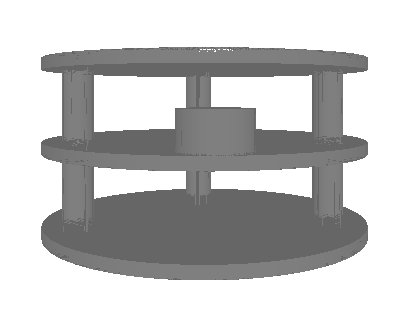
\includegraphics[width=200pt]{img/3morduc_opengl.png}  %robot pic
    \caption{The 3morduc robotic platform drawn in OpenGL}
    \label{fig:3morduc_opengl}
  \end{center}
\end{figure}
%
The default \texttt{radius} value is 4, but it can be 
customised by the user: by increasing it the robot will be 
displayed larger and larger on the screen, and viceversa.
%

%
All the attributes are private in the new robot class, 
so a method to get each one value is declared. 
%

%
Most of the previous public methods have been removed too. 
The constructor method, for instance, is present with one
only definition and default parameters, instead of declaring 
it twice (with parameter and without). The methods to set
linear and angular velocity are not present anymore, for 
the reason explained above; those to increment the collisions 
number are actually disabled because, at this development 
stage, the exocentric vision control does not face the collision 
problem. Anyway, it is supposed to cope with collision in 
the future version.
%

%
Besides, the method used by Privitera's simulator to read 
the robot initial position from file has been removed, since 
for the exocentric vision system robot always starts from 
fixed coordinates and rotation.
%

%
Finally, the method named with the signature 
\texttt{void move()} has been changed in \texttt{void Place(float x, float y, float theta)}
in order to set the x and y coordinate and the rotation of the robot. 
We remind that in the previous version these attributes
were public, so there were no need to pass them as parameters function.

\subsubsection{The Camera Class}
\label{sub:cameraclass}


First of all, there is no thing like a camera in OpenGL, therefore we have to
simulate one.
%

%
A camera object allows to move and rotate the user point of view and robot
object independently, avoiding that one interferes the other. For the exocentric
vision application this is a basic feature, because robot can be placed
everywhere in OpenGL world regardless of the camera position, and viceversa.
%

%
The camera object implementation has been suggested by \cite{opengl:camera}.
It provides some elementary commands implemented by means of mathematical matrix
operations, to move the camera or rotate it along one axis.

\subsection{How to choose the right background image}
\label{sub:howbackgroundimage}

There are many ways of choosing the background image among the collected ones. This unique
block, entitled "choose K" in diagram \ref{fig:overall_diagram}, can be thought of as a
black box, with the robot position and orientation data as input and the background image
(or better, its path) as output.
%

%
To make easier the definition and the deployment of a new algorithm, the interface
\texttt{DistanceCalcInterface} has been declared, with only one pure virtual method named
\texttt{Calculate}. Every new algorithm able to choose a background image has to be defined
within the \texttt{Calculate} function.
\texttt{Calculate} return a float value, that is a score value; the parameters taken are a
single image and the robot data. When the robot changes its position or orientation, the
framework built computes the \texttt{Calculate} function for every image, with the new robot
values. Every image is therefore coupled with a score, and the one with minimum associated value
will be chosen.
%

%
All you need to run a different algorithm is to instance the right object implementing the
\texttt{DistanceCalcInterface} and link it with the \texttt{DataManager}, who will automatically
use the custom function to evaluate the score for every stored image. As written before, the
one with the lowest score will be rendered as background texture.
%

%
For instance, if the target is to select the image shoot closest to the actual robot position,
the returned score will be the euclidean distance between the image and robot itself. In this way
the minimum score will be associated with the closest image.
The algorithm described above is implemented within the \texttt{Calculate} function of the
\texttt{SpacialMetricCalc} class (see class diagram \ref{fig:class_diagram} and chapter
\ref{subsec:spacial_metric_algorithm}).
%

%
Another class, named \texttt{SweepMetricCalc}, implements the
\newline
\texttt{DistanceCalcInterface}, but it defines a totally different and more complex algorithm.
Chapter \ref{subsec:sweep_metric_algorithm} will explain it in detail.

\subsection{How to retrieve data}
\label{sub:howretrievedata}
